\documentclass[letterpaper,11pt,twocolumn]{article}

%%%%%%%%%%%%%%%%%%%%%
% Packages

\usepackage{amsmath} % includes basic math fonts
\usepackage{amsthm}  % includes basic math environments
\usepackage{graphicx} % allows inclusion of images

\usepackage{lipsum} % for generating filler text

\usepackage{titling} % custom title height
\setlength{\droptitle}{-5.8em}

%%%%%%%%%%%%%%%%%%%%%
% Define math environments (You can add your own environments)
 
\newtheorem{definition}{Definition}
\newtheorem{theorem}{Theorem}

%%%%%%%%%%%%%%%%%%%%%
% Title information


\title{A Brief Comprehension of the Heuristic Algorithm}
\author{Junze Tan}
\date{December 2021}

%%%%%%%%%%%%%%%%%%%%%
% Beginning of document
\begin{document}

\maketitle % this displays the title information.

\section{Abstract}
The aim of this expository report is to explain and analyze the Heuristic Algorithm which is for the Steiner tree problem in a undergraduate-understandable way. Furthermore, there will be some extensions of this algorithm like, application, related algorithm in this report. Besides, we will not talk about the time complexity of this algorithm which exceed the knowledge that we learned in Graph theory.


\section{Introduction}
Before the analysis, there are some notations and basic background information that readers need to know.\\
According to the article from Networks, Steiner tree problem is to find a tree of G that spans S with minimal total distance on its edges. \cite{treeProb}\\
Given an complete undirected distance graph G = (V, E, d) where V is the set of vertices, E is the set of edges, d is a distance function which maps E into the set of non-negative numbers.\\
A set S $\subseteq$ V is a subset of the distinguished vertices of V which we shall call Steiner Points \\
The minimal spanning tree of G is a spanning tree (we learned from class) such that the total distance on its edges is minimal among all spanning trees.\cite{treeProb}

\section{Analysis}
First, Let us know what is a Heuristic Algorithm. When we are facing a Steiner tree problem, the Heuristic Algorithm produced a Steiner tree as we input the set of Steiner points S. \cite{main} Notice that, the Steiner tree produced is not necessarily minimal, however, the total distance of this tree is very close to the distance of minimal Steiner tree.\\
Then, we can go through Heuristic Algorithm. To begin with, we need in put a undirected graph G = (V, E, d) and Steiner points S.
\subsection{implementation steps}
By the results from \cite{main}, we can implement the algorithm as the following.
\begin{itemize}
    \item Step 1: Construct the complete undirected distance graph $G_1 = (V_1, E_1, d_1)$ from G and S.
    \item Step 2: Find the minimal spanning tree, $T_1$, of $G_1$. (In case there are several minimal spanning trees, pick an arbitrary one.)
    \item Step 3: Construct the subgraph, $G_s$, of G by replacing each edge in $T_1$ by its corresponding shortest path in G. (In case there are several shortest paths, pick an arbitrary one.)
    \item Step 4: Find the minimal spanning tree, $T_s$, of $G_s$. (If there are several minimal spanning trees, pick an arbitrary one.)
    \item Step 5: Construct a Steiner tree, $T_H$ from $T_s$ by deleting edges in $T_s$, if necessary, so that all the leaves in $T_H$ are Steiner points.
\end{itemize}

\subsection{Example}
Here is a example from \cite{main}.\\
Given an complete undirected distance graph G = (V, E, d) with Steiner points $S = {v_1, v_2, v_3, v_4}$\\
\begin{center}
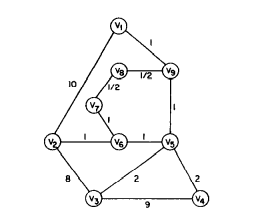
\includegraphics[scale = 0.8]{a.png}\\
\end{center}
1. Construct $G_1$ from G and S.\\
\begin{center}
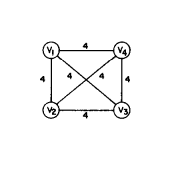
\includegraphics[scale = 0.8]{b.png}\\    
\end{center}
2. Find the minimal spanning tree.\\
\begin{center}
    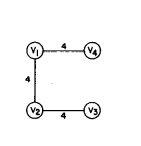
\includegraphics[scale = 0.8]{c.png}
\end{center}
3. Construct $G_s$ by replacing each edge in $T_1$ by its corresponding shortest path in G.
\begin{center}
    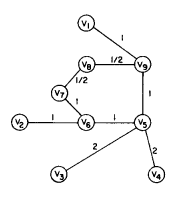
\includegraphics[scale = 0.8]{d.png}
\end{center}
4. Find the minimal spanning tree, $T_s$, of $G_s$.
\begin{center}
    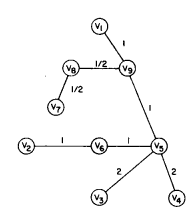
\includegraphics[scale = 0.8]{e.png}
\end{center}
5. Construct a Steiner tree, $T_H$ from $T_s$.
\begin{center}
    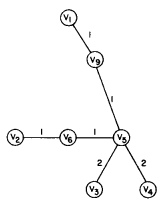
\includegraphics[scale = 0.8]{f.png}
\end{center}\\
\begin{flushleft}
Finally the Steiner Tree $T_s$ is generated as the last graph above.\\
\end{flushleft}

\section{Summary}
Basically, this algorithm provides a faster and efficient way to get the result. Nevertheless, there are still some disadvantages like lack of optimality, inaccuracy, imprecision, or incompleteness for speed. In our real life, Heuristic Algorithm have many application in various areas. There is a well-known example. Traveling Salesmen Problem is a famous problem that can be solved by Heuristic Algorithm. The problem is as follows: given a list of cities and the distances between each city, what is the shortest possible route that visits each city exactly once? \cite{Salesman} So that we can use Heuristic Algorithm to solve it.\\
There is another algorithm by Kurt Mehlhorn which improved Heuristic Algorithm we discussed. See from \cite{approxi}. He change algorithm from the original one. \\ 
\begin{itemize} 
    \item First let us construct complete distance graph $G_1 = (V_1,E_1,d_1)$, where $V_1 = S$ and, for every $(v_i, v_j \in E_1$, $d_1(v_i,v_j)$ is equal to the distance of a shortest path from $v_i$ to $v_j$ in G. 
    \item For step 2, finding  a minimum spanning tree $G_2$ of $G_1$. 
    \item Then, Construct a subgraph $G_3$ of G by replacing each edge in $G_2$ by its corresponding shortest path in G, and find a minimum spanning tree $G_4$ of $G_3$. 
    \item Finally, construct a Steiner tree $G_5$ from $G_4$ by deleting edges in $G_4$. 
\end{itemize}    
This algorithm is simpler than the Heuristic Algorithm. That's a brief explanation of Kurt's approximation algorithm. There are still many applications and extension that related with Heuristic Algorithm that did not listed. \\
Finally, There is a question. Why we use Heuristic algorithm in stead of exact algorithm. One of the reason is that Heuristic algorithm is efficient than the exact algorithm in the situation which do not require precision and accuracy. Also, Heuristic algorithm is often used in case of approximate solutions are sufficient. So that we do not have to find the exact solutions that are computationally expensive.


% The bibiliography
\begin{thebibliography}{1}

\bibitem{main} 
Kou, L., Markowsky, G. & Berman, L. 
\textit{A fast algorithm for Steiner trees}. 
Acta Informatica, journal, 1(15):141-145, 1981.

\bibitem{treeProb} 
Dreyfus, S. E. and Wagner, R. A.
\textit{The steiner problem in graphs}. 
Networks, journal, 3:195-207, 1971.

\bibitem{Salesman} 
Gutin, G. and Punnen, A.P.
\textit{The Traveling Salesman Problem and Its Variations}. 
Combinatorial Optimization, book, Springer US, 2006.

\bibitem{approxi} 
Kurt Mehlhorn
\textit{A faster approximation algorithm for the Steiner problem in graphs}. 
Information Processing Letters, journal, 27(3):125-128, 1988.

\end{thebibliography}





\end{document}
